%% Copyright (c) 2022 Martín E. Zahnd
%%
%% This code is licensed under MIT license (see LICENSE.txt for details)
%%
\chapter{Lógica de Primer Orden}
\graphicspath{ {./teoria/resources/logica-primer-orden/} }

\section{Lenguaje}

\subsection{Alfabeto}
La lógica de primer orden es un lenguaje de primer orden, por esto, es 
necesario comenzar definiendo un alfabeto.

\begin{definicion}{Alfabeto}{}
    El alfabeto que utilizamos para lógica de primer orden se define como:

    \begin{gather*}
        A_{\mathcal{F}, \mathcal{C}, \mathcal{P}} =
        \mathrm{VAR}
        \cup \mathrm{ CONECTIVOS }
        \cup \{\;(\;,\; )\;\}
        \cup \mathcal{F}
        \cup \mathcal{C}
        \cup \mathcal{P}
    \end{gather*}

    \medskip

    Donde:
    
    \begin{itemize}
    \item $\mathrm{VAR} = \{ x_0, x_1, x_2, \dots \}$

    \bigskip
    \textbf{Notación:}
    $x_i, y_i, z_i, w_i$

    \item $\mathrm{CONECTIVOS } = \{ \wedge,\vee,\to,\neg \} \cup 
        \{ \forall, \exists \}$
    \nota{$\forall$: Cuantificador universal.\\
        $\exists\,$: Cuantificador existencial.}%

    \item $\mathcal{F} =$ es un conjunto cuyos elementos se llaman símbolos de 
    función. 
    $\mathcal{F}$ podría ser vacío.

    \bigskip
    \textbf{Notación:}
    $f_i^k, g_i^k, h_i^k$
    \nota{$k$ se denomina ``aridad''}%

    \item $\mathcal{C} = $ es un conjunto cuyos elementos se llaman símbolos de
    constantes.
    Podría ser vacío.

    \bigskip
    \textbf{Notación:}
    $c_i, d_i, k_i$

    \item $\mathcal{P} = $ es un conjunto cuyos elementos se llaman símbolos de
    predicado. $\mathcal{P} \neq \varnothing$

    \bigskip
    \textbf{Notación:}
    $P_i^k, Q_i^k, R_i^k$
    \nota{$k$ se denomina ``aridad''}%
    \end{itemize}
\end{definicion}

Notemos que $\mathrm{VAR}$ y los $\mathrm{CONECTIVOS}$ son siempre los mismos, 
mientras que $\mathcal{F}, \mathcal{C}, \mathcal{P}$ pueden variar. Por ello,
estamos definiendo infinitos alfabetos que dependen de estos tres conjuntos.


\subsection{Término y fórmula}

\begin{definicion}{Término a partir de un alfabeto}{}
    Sea $A$ un alfabeto.

    \medskip

    \begin{enumerate}
        \item Toda variable es un término.
        \item Toda constante es un término.
        \item Si $t_1, t_2, \dotsc, t_k$ son términos y $f^k \in \mathcal{F}$
            \begin{gather*}
                \implies f^{k} (t_1,t_2,\dotsc,t_k) \text{ es un término}
            \end{gather*}
        \item Cualquier expresión de $A^{*}$ que se obtiene aplicando
            finitas veces (1), (2) y (3) es un término.
    \end{enumerate}
    
    \bigskip
    \textbf{Notación:}
    $ \mathrm{TERM}$
\end{definicion}

\medskip 

\begin{definicion}{Término cerrado}{}
    Un término se llama cerrado si no tiene variables.
\end{definicion}

\medskip 

\begin{definicion}{Fórmula a partir de un alfabeto}{}
    Sea $A$ un alfabeto.

    \medskip

    \begin{enumerate}
        \item Si $t_1, \dotsc, t_k \in  \mathrm{TERM}$ 
            y $P^{k} \in \mathcal{P}$
                $\implies P^{k}(t_1, \dotsc, t_k)$ es una fórmula.

            Esta se denomina \textit{fórmula atómica}.
        \item $\alpha \in \mathrm{FORM}$
            $\implies \neg \alpha \in \mathrm{FORM}$

        \item $\alpha, \beta \in \mathrm{FORM}$
            $\implies (\alpha\wedge\beta),(\alpha\vee\beta),
            (\alpha\to\beta) \in \mathrm{FORM}$
        \item $\alpha \in \mathrm{FORM}$, $x \in \mathrm{VAR}$
            \nota{$\forall x$ [espacio] $\alpha$}%
            $\implies \forall x \quad \alpha \in \mathrm{FORM}$
        \item $\alpha \in \mathrm{FORM}$, $x \in \mathrm{VAR}$
            \nota{$\exists\; x$ [espacio] $\alpha$}%
            $\implies \exists\; x \quad \alpha \in \mathrm{FORM}$
        \item Cualquier expresión de $A^{*}$ que se obtiene aplicando
            finitas veces (1), (2), (3), (4) y (5) es una fórmula.
    \end{enumerate}

    \bigskip
    \textbf{Notación:}
    $F = \mathrm{FORM}$
\end{definicion}

\subsubsection{Ejemplos}

\subsubsection{\underline{Términos}}

\begin{multicols}{2}
    \begin{itemize}
            \item $x_1$
            \item $h^{2}(c,d)$ \nota{Este término, $h^2$, en particular 
                es cerrado}%
            \item $c_2$
            \item $f^{3} (c_1, x_1, x_2)$
            \item $g^{2}(x_1, f^{3}(c_1, x_1, x_2))$
            \item[\vspace{\fill}]
    \end{itemize}
\end{multicols}


\subsubsection{\underline{Fórmulas}}

\begin{itemize}
        \item $\forall x_1 \quad (P^{3}(x_1, x_2, c_1) 
            \to Q^{1}(f^{3}(c_1,x_1,x_2)))$
    \begin{multicols}{2}
        \item $P^{2}(x_1, c_2)$
        \item $\neg P^{2} (x_1, x_2)$
        \item $\exists \; x_1 \quad P^{2}(x_1,x_2)$
        \item[\vspace{\fill}]
    \end{multicols}
\end{itemize}


\section{Sintaxis} % Creo que es a partir de acá. Verificar.

\subsection{Lenguaje de primer orden}

\begin{definicion}{Lenguaje de 1\textsuperscript{er.} orden}{}
    Dado un alfabeto $A$, $\mathcal{L} \subseteq A^{*}$ es un lenguaje
    de primer orden si
    \begin{gather*}
        \mathcal{L} = \mathrm{FORM} \cup \mathrm{TERM}
    \end{gather*}

    \bigskip
    \textbf{Notación:}
    $\mathcal{L} = <\mathcal{C}, \mathcal{F}, \mathcal{P}>$
\end{definicion}


\subsection{Variables libres, ligadas y enunciados}

Para ayudarnos a comprender las definiciones que presentaremos a continuación,
veamos primero los siguiente ejemplos.

\begin{itemize}
    \item $\forall x \quad \beta$ \nota{$\beta \in F, x \in \mathrm{VAR}$}%

        El alcance con que cuantifique $x$ el $\forall$ es en $\beta$.

    \item $(\forall x \quad \beta \to \gamma)$

        El cuantificador tiene alcance sobre $\beta$ pero no sobre $\gamma$.

    \item $\forall x \quad (\beta \to \gamma)$

        El cuantificador tiene alcance sobre $\beta$ y $\gamma$.
\end{itemize}

\begin{definicion}{Variables ligadas}{}
    Una aparición de una variable $x$ en una fórmula está ligada si es 
    alcanzada por un cuantificador.

    \smallskip

    Una variable es ligada en una fórmula si todas sus apariciones son ligadas.

\end{definicion}

\medskip

\begin{definicion}{Variables libres}{}
    Una aparición de una variable $x$ en una fórmula es libre si no esta
    ligada. 

    \smallskip

    Una variable es libre en una fórmula si todas sus apariciones son libres.
\end{definicion}

\medskip

\begin{definicion}{Enunciado}{}
    Una fórmula se llama \textit{enunciado} o \textit{sentencia} si todas sus 
    variables están ligadas.
\end{definicion}


\subsubsection{Ejemplos}

\begin{enumerate}
    \item $\alpha = P(x_1, x_2)$

        $x_1$ y $x_2$ están libres.

    \item $\alpha = \forall x_1 \quad P(x_1, x_2)$

        $x_1$ es ligada, $x_2$ es libre.

    \item $\alpha = (\underbrace{\forall x_1 \quad P(x_1, x_2)}_{\circled{1}}
        \to \underbrace{P(x_2, x_1)}_{\circled{2}})$

        En \circled{1}, $x_1$ es ligada; $x_2$ es libre.

        En \circled{2}, $x_1$ y $x_2$ están libres.

        Como $x_1$ tiene una aparición libre y otra ligada, decimos que $x_1$
        no es libre ni ligada; y $x_2$ es libre.

    \item $\alpha = \forall x_1 \quad \exists\; x_2 \quad P(x_1, x_2)$

        $\alpha$ es un enunciado pues todas las variables están ligadas.
\end{enumerate}

\section{Semántica}

\begin{definicion}{Interpretación}{}
    Dado \underline{un} alfabeto $A$ y un lenguaje $\mathcal{L}$ de primer
    orden, una interpretación $\mathcal{I}$ de $\mathcal{L}$ consiste en:

    \begin{enumerate}
        \item $\mathcal{U} \neq \varnothing$

            Siendo $\mathcal{U}$ un conjunto llamado \textit{universo}.

        \item Si $c \in \mathcal{C}$, entonces $c$ se interpreta como 
            $c_{\mathcal{I}} \in \mathcal{U}$.

        \item $f^{k} \in \mathcal{F}$, entonces $f^{k}$ se interpreta como una
            función cuyo dominio es $\mathcal{U}^{k}$ y el codominio
            $\mathcal{U}$. 
            \nota{$f_\mathcal{I}^{k}: \mathcal{U}^k \to \mathcal{U} $}%
    
        \item $P^k \in \mathcal{P}$, entonces $P^k$ se
            interpreta como una relación $k\mathrm{-}aria$ en $\mathcal{U}$.
            Es decir, $P_\mathcal{I}^{k} \subseteq \mathcal{U}^k$
    \end{enumerate}

    \medskip

    $\mathcal{I}$ se llama \textit{interpretación de $\mathcal{L}$} o
   $\mathcal{L}\mathrm{-}estructura$.
\end{definicion}

\subsubsection{Ejemplos}

Sea $\mathcal{L}$ un lenguaje de 1\textsuperscript{er.} orden tal que:

\begin{center}
    \begin{tabular}{c c c}
        $\mathcal{C} = \{ c,d \}$ & $\mathcal{F} = \{ f^3 , g^2 \}$
        & $\mathcal{P} = \{ P^2 \}$
    \end{tabular}
\end{center}

\begin{enumerate}
    \item Sea 

    \begin{align*}
        \mathcal{I}_1 = (\;
        &\mathcal{U}_{\mathcal{I}_1} = \mathbb{Z}, \quad
        c_{\mathcal{I}_1} = 2, \quad
        d_{\mathcal{I}_1} = -1, \\
        &f_{\mathcal{I}_1}^3 (x,y,z) = x+y-z, \quad
        g_{\mathcal{I}_1}^2 (x,y) = xy, \\
        & P_{\mathcal{I}_1}^2 = \{ (x,y)/ x \equiv y (3) \}
        \subseteq \mathbb{Z}^{2} = \mathcal{U}^{2}
        \;)
    \end{align*}

    \medskip

    ¿Es $\mathcal{I}_1$ una interpretación de $\mathcal{L}$? Sí pues:

    \begin{itemize}[label=\cmark]
        \item $\mathcal{U}_{\mathcal{I}_1} = \mathbb{Z} \neq \varnothing$
        \item  $c_{\mathcal{I}_1} = 2 \in \mathbb{Z}$
        \item  $d_{\mathcal{I}_1} = -1 \in \mathbb{Z}$
        \item  $Dom(f_{\mathcal{I}_1}^3) = \mathbb{Z}^3$
        \item  $Codom(f_{\mathcal{I}_1}^3) = \mathbb{Z}$
        \item  $Dom(g_{\mathcal{I}_1}^2) = \mathbb{Z}^2$
        \item  $Codom(g_{\mathcal{I}_1}^2) = \mathbb{Z}$
        \item  $\mathcal{P} \subseteq \mathbb{Z} \times \mathbb{Z}$
    \end{itemize}

    \item Sea 

        \begin{gather*}
        \mathcal{I}_2 = (\mathcal{U}_{\mathcal{I}_2} = \mathbb{N}, \;
        c_{\mathcal{I}_2} = 0, \;
        d_{\mathcal{I}_2} = 3, \;
        f_{\mathcal{I}_2}^3 (x,y,z) = x+y, \\
        g_{\mathcal{I}_2}^2 (x,y) = \nicefrac{x}{y}, \;
        P_{\mathcal{I}_2}^2 = \{ (x,y)/ xy=yx \}
        ) 
    \end{gather*}

    \medskip

    ¿Es $\mathcal{I}_2$ una interpretación de $\mathcal{L}$? ¡No!

    \begin{itemize}[label=\cmark]
        \item $\mathcal{U}_{\mathcal{I}_2} = \mathbb{N} \neq \varnothing$
        \item  $c_{\mathcal{I}_2} = 0 \in \mathbb{N}$
        \item  $d_{\mathcal{I}_2} = 3 \in \mathbb{N}$
        \item  $Dom(f_{\mathcal{I}_2}^3) = \mathbb{N}^3$
        \item  $Codom(f_{\mathcal{I}_2}^3) = \mathbb{N}$
        \item[\xmark]  $Dom(g_{\mathcal{I}_2}^2) 
            = \mathbb{N} \times \left(\mathbb{N} - \{ 0 \}\right)
            \neq \mathbb{N}^2$: 
            Pues $g_{\mathcal{I}_2}^{2}(3,0)$ no está definida.
    \end{itemize}
\end{enumerate}

\subsection{Valuaciones}

\begin{definicion}{Valuación}{}
    Dado un lenguaje de primer orden y una interpretación $\mathcal{I}$ de
    $\mathcal{L}$, definimos valuación como una función 
    $v: \mathrm{VAR} \to \mathcal{U}_{\mathcal{I}}$.
\end{definicion}

\medskip

¿Cómo interpretamos los términos?

Definamos para ello una extensión de $v$.

\begin{definicion}{Valuación extendida}{}
    Dada $v$ una valuación, definimos
    $\bar{v}: \mathrm{TERM} \to \mathcal{U}_{\mathcal{I}}$ 
    que verifica:

    \begin{enumerate}
        \item $\bar{v} (x_i) = v(x_i)$ 
            \nota{$x_i \in \mathrm{VAR}$}%
        \item $\bar{v}(c) = c_{\mathcal{I}}$ 
            \nota{$c \in \mathcal{C}$}%
        \item $\bar{v}( f^{k}(t_1, \dotsc, t_k)) = 
            f_{\mathcal{I}}^{k}(\bar{v}(t_1), \dotsc, \bar{v}(t_k))$
            \nota{$f^{k} \in \mathcal{F}$ y 
            $t_1, \dotsc, t_k \in \mathrm{FORM}$}%
    \end{enumerate}

    Entonces decimos que $\bar{v}$ es extensión de $v$.
\end{definicion}

\medskip

\begin{definicion}{Valuación modificada}{}
    Dada $v$ valuación, definimos valuación modificada como:
    \begin{gather*}
        v_{x_{1} = a}: \mathrm{VAR} \to \mathcal{U}_{\mathcal{I}} / 
        v_{x_{1}=a}(x) =
        \begin{cases}
            v(x) & \text{si } x \neq x_1 \\
            a & \text{si } x = x_1
        \end{cases}
    \end{gather*}
\end{definicion}

\subsubsection{Ejemplo}

Sea $\mathcal{L}$ de 1\textsuperscript{er.} orden, con $\mathcal{C}=\{c\}$,
$\mathcal{F}=\{ f^{2} \}$, $\mathcal{P}=\{ P^{2} \}$

Sea 
\begin{align*}
    \mathcal{I} &= (\mathcal{U}_{\mathcal{I}} = \mathbb{Z}, \quad
            c_{\mathcal{I}} = 0, \quad
            f_{\mathcal{I}}^2 (x,y) = x+y, \quad
            P_{\mathcal{I}} = \{ (x,y)/ x \equiv y (2) \}
    ) \\
    &= ( \mathbb{Z}, ~
    0, ~
    +, ~
    \{ (x,y) / x \equiv y (2) \} )
\end{align*}

Sea $v: \mathrm{VAR} \to \mathbb{Z} / v(x_i) = 2i$

Sean $t_1 = f^{2} (x_1, x_3)$ y $t_2 = f^{2} (x_5, c)$

\underline{Se pide hallar $\bar{v}(t_1)$ y $\bar{v} (t_2)$}

\medskip

\begin{align*}
    \bar{v}(t_1) &= f_{\mathcal{I}}^{2}(\bar{v}(x_1), \bar{v}(x_3)) \\
                 &= \bar{v}(x_1) + \bar{v}(x_3) \\
                 &= v(x_1) + v(x_3) \\
                 &= 2\, . \, 1 + 2 \, . \, 3 \\
                 &= 8 
\end{align*}
\begin{align*}
    \bar{v}(t_2) &= f_{\mathcal{I}}^{2}(\bar{v}(x_5), \bar{v}(c)) \\
                 &= \bar{v}(x_5) + \bar{v}(c) \\
                 &= v(x_5) + c_{\mathcal{I}} \\ 
                 &= 2\, . \, 5 + 0 \\
                 &= 10
\end{align*}

\subsection{Valor de verdad para las fórmulas}

¿Cómo asignamos un valor de verdad a las fórmulas?

Veamos primero la notación para ello y, luego, la definición del valor de 
verdad para las fórmulas.
\begin{definicion}{Fórmula verdadera y falsa}{}
    Sean $\mathcal{L}$ un lenguaje de 1\textsuperscript{er.} orden,
    $v: \mathrm{VAR} \to \mathcal{U}_{\mathcal{I}}$,
    $\alpha \in \mathrm{FORM}$ y \\
    $V_{\mathcal{I}, v(\alpha)}: \mathrm{FORM} \to \{ 0,1 \}$
    \begin{itemize}
        \item $\alpha$ es \textit{verdadera} en la interpretación 
            $\mathcal{I}$ con valuación $v$:

            \textbf{Notación:}
            \nota{Ambas notaciones son equivalentes}%
            \begin{multicols}{2}
                \begin{itemize}
                    \item $V_{\mathcal{I}, v}(\alpha) = 1$
                    \item $\mathcal{I} \vDash \alpha [v]$
                \end{itemize}
            \end{multicols}

        \item $\alpha$ es \textit{falsa} en la interpretación 
            $\mathcal{I}$ con valuación $v$:

            \textbf{Notación:}
            \nota{Notaciones equivalentes}%
            \begin{multicols}{2}
                \begin{itemize}
                    \item $V_{\mathcal{I}, v}(\alpha) = 0$
                    \item $\mathcal{I} \nvDash \alpha [v]$
                \end{itemize}
            \end{multicols}
    \end{itemize}
\end{definicion}

\begin{definicion}{Fórmula satisfacible y válida}{}
    Sea $\mathcal{L}$ un lenguaje de 1\textsuperscript{er.} orden.

    Sea $v: \mathrm{VAR} \to \mathcal{U}_{\mathcal{I}}$.

    Sea $\alpha \in \mathrm{FORM}$.

    Sea $V_{\mathcal{I}, v}(\alpha): \mathrm{FORM} \to \{ 0,1 \}$
    \begin{itemize}
        \item $\alpha$ es \textit{satisfacible} si existe una interpretación 
            $\mathcal{I}$  y una valuación $v$ que la hacen verdadera.

            \bigskip
            \textbf{Notación:}
            $V_{\mathcal{I}, v}(\alpha) = 1$ ó $\mathcal{I} \vDash \alpha [v]$

        \item $\alpha$ es \textit{válida} en una interpretación
            $\mathcal{I}$ si es verdadera para
            toda $v$ valuación.

            También podemos decir que $\mathcal{I}$ es un \textit{modelo} 
            para $\alpha$.

            \bigskip
            \textbf{Notación:}
            $\mathcal{I} \vDash \alpha$

        \item $\alpha$ es \textit{universalmente válida} si 
            $V_{\mathcal{I}, v}(\alpha) = 1$ para todo $\mathcal{I}$ y para 
            toda $v$ valuación.

            \bigskip
            \textbf{Notación:}
            $\vDash \alpha$
    \end{itemize}
\end{definicion}

\medskip

\begin{definicion}{Valor de verdad para las fórmulas}{}
Dado $\mathcal{L}$ de 1\textsuperscript{er.} orden, $\mathcal{I}$ de 
$\mathcal{L}$, $v: \mathrm{VAR} \to \mathcal{U}_{\mathcal{I}}$.

Sea $V_{\mathcal{I}, v}(\alpha): \mathrm{FORM} \to \{ 0,1 \}$

Los casos en que $\alpha$ es verdadero o falso son los siguientes:
\begin{enumerate}
    \item $\alpha = P^{k} (t_1, \dotsc, t_k)$
        \nota{$P^k \in \mathcal{P}$,
        $t_j \in  \mathrm{TERM}$ con $1\leq j \leq k$}%
        \begin{gather*}
            V_{\mathcal{I}, v}(\alpha) = 1 \iff 
            (\bar{v}(t_1), \bar{v}(t_2), \dotsc, \bar{v}(t_k)) 
            \in P^{k}_{\mathcal{I}}
        \end{gather*}

        \nota{Notemos que todo
            $\bar{v}(t_i) \in \mathcal{U}_{\mathcal{I}}$, $1\leq i \leq k$}%
    \item $\alpha = \neg \beta$ 
        \begin{gather*}
            \notamath{$\beta \in \mathrm{FORM}$}
            V_{\mathcal{I}, v}(\alpha) = 1 - V_{\mathcal{I}, v}(\beta)
        \end{gather*}

    \item $\alpha=(\beta_1 \wedge \beta_2)$
        \nota{$\beta_1, \beta_2 \in \mathrm{FORM}$}%
        \begin{gather*}
            V_{\mathcal{I}, v}(\alpha) = \min 
            \{V_{\mathcal{I}, v}(\beta_1), V_{\mathcal{I}, v}(\beta_2)\}
        \end{gather*}

    \item $\alpha = (\beta_1 \vee \beta_2)$
        \begin{gather*}
            V_{\mathcal{I}, v}(\alpha) = \max
            \{ V_{\mathcal{I}, v}(\beta_1), V_{\mathcal{I}, v}(\beta_2) \}
        \end{gather*}

    \item $\alpha = (\beta_1 \to \beta_2)$
        \begin{gather*}
            V_{\mathcal{I}, v}(\alpha) = \max
            \{ 1-V_{\mathcal{I}, v}(\beta_1), V_{\mathcal{I}, v}(\beta_2) \}
        \end{gather*}

    \item $\alpha = \forall x_i \quad \beta$
        \nota{$\beta \in \mathrm{FORM}$, $x_i \in \mathrm{VAR}$\\
        El valor de verdad es 1 si es verdadero en $\beta$ sin importar $x_i$. 
        No importa qué hace la valuación original en $x_i$, solo importa qué
        hace la de $\beta$.}%
        \begin{gather*}
            V_{\mathcal{I}, v}(\alpha) = 1 \iff
            V_{\mathcal{I}, v_{x_i=a}}(\beta) = 1
        \end{gather*}
        Para todo elemento $a \in \mathcal{U}_{\mathcal{I}}$.
    \item $\alpha = \exists x_i \quad \beta$
        \begin{gather*}
            V_{\mathcal{I}, v}(\alpha) = 1 \iff
            V_{\mathcal{I}, v_{x_i=a}}(\beta) = 1
        \end{gather*}
        Para algún $a \in \mathcal{U}_{\mathcal{I}}$.
\end{enumerate}     
\end{definicion}

\bigskip
    \textit{Observación:}
    Si $\alpha$ es enunciado, entonces $V_{\mathcal{I}, v}(\alpha)$ no depende
    de $v$.

    Es decir, si cambiamos $v$ por $w$ valuación $\implies$ 
    \nota{$\forall v, w$ valuación}%
    $V_{\mathcal{I}, v}(\alpha) = V_{\mathcal{I}, w}(\alpha)$

    \subsubsection{Ejemplos}

    \begin{itemize}
        \item Dado $\mathcal{I} = ( \mathbb{Z}, \;
            0 , \;
            + , \;
            \{ (x,y)/x \equiv y(2) \})$,
        $v: \mathrm{VAR} \to \mathbb{Z} / v(x_i) = 2i$
        
        \underline{Hallar $V_{\mathcal{I}, v} (\alpha)$ }
        
        \begin{enumerate}
            \item $\alpha = P(x_1, x_4)$
                \begin{align*}
                    V_{\mathcal{I}, v}(\alpha) &= 1  \\
                    &\iff (\bar{v}(x_1), \bar{v}(x_4)) \in P_{\mathcal{I}} \\
                    &\iff \bar{v}(x_1) \equiv \bar{v}(x_4) \; (2) \\
                    &\iff v(x_1) \equiv v(x_4) \; (2) \\
                    &\iff 2 \, . \, 1 \equiv 2 \, . \, 4 \; (2) \\
                    &\iff 0 \equiv 0 \; (2)
                \end{align*}
        
                \begin{gather*}
                    \dashbox{$\therefore ~ V_{\mathcal{I},v} (\alpha) = 1$}
                \end{gather*}
        
            \item $\alpha = \forall x_1 \quad \forall x_2 \quad P(x_1, x_2)$
                \begin{align*}
                    V_{\mathcal{I}, v}(\alpha) &= 1  \\
                    &\iff V_{\mathcal{I}, {v_{x_1 = a}}}
                        (\forall x_2 \quad P(x_1,x_2)) = 1
                    \notamath{$\forall a \in \mathcal{U}_{\mathcal{I}}$}\\
                    &\iff V_{\mathcal{I}, {v_{x_1 = a, x_2 = b}}} (P(x_1,x_2))=1 \\
                    &\iff (\bar{v}_{x_1 = a, x_2 = b} (x_1),
                    \bar{v}_{x_1 = a, x_2 = b} (x_2)) \in P_{\mathcal{I}} 
                    \notamath{$\forall a \in \mathcal{U}_{\mathcal{I}}$,
                    y $\forall b \in \mathcal{U}_{\mathcal{I}}$}  \\
                    &\iff v_{x_1 = a, x_2 = b} (x_1) \equiv 
                    v_{x_1 = a, x_2 = b} (x_2) \; (2) \\
                    &\iff a \equiv b \; (2)
                    \notamath{$\forall a \in \mathcal{U}_{\mathcal{I}}$,
                    y $\forall b \in \mathcal{U}_{\mathcal{I}}$}  \\
                \end{align*}
        
                Es falso pues basta tomar $a=1$, $b=0$ y $1 \not\equiv 0 \; (2)$
                \begin{center}
                    \dashbox{$\therefore ~ V_{\mathcal{I},v} (\alpha) = 0$}
                \end{center}
        
            \item $\alpha = \forall x \quad \exists \; y \quad P(x,y)$
                \begin{align*}
                    V_{\mathcal{I}, v}(\alpha) &= 1  \\
                    &\iff V_{\mathcal{I}, v_{x=a}}(\exists \quad P(x,y)) = 1
                    \notamath{$\forall a \in \mathcal{U}_{\mathcal{I}}$} \\
                    &\iff V_{\mathcal{I}, v_{x=a, y=b}}(P(x,y)) = 1
                    \notamath{$\forall a \in \mathcal{U}_{\mathcal{I}}$ existe
                    $b \in \mathcal{U}_{\mathcal{I}}$} \\
                    &\iff \text{Dado $a \in \mathcal{U}$, existe } 
                    b \in \mathcal{U} /
                    a \equiv b (2)
                \end{align*}
        
                Esto es verdadero pues basta tomar $b=a$.
                \begin{gather*}
                    \dashbox{$\therefore ~ V_{\mathcal{I},v} (\alpha) = 1$}
                \end{gather*}
        
            \item $\exists \; y \quad \forall x \quad P(x,y)$
                \begin{align*}
                 V_{\mathcal{I}, v}(\alpha) &= 1  \\
                    &\iff V_{\mathcal{I}, v_{y=b}}(\forall x \quad P(x,y)) = 1
                    \notamath{Para algún $b \in \mathcal{U}_{\mathcal{I}}$} \\
                    &\iff \text{Fijando algún $b$ en $\mathcal{U}_{\mathcal{I}}$, }
                    V_{\mathcal{I}, v_{y=b,x=a}}(P(x,y)) = 1
                    \notamath{Para todo $a \in \mathcal{U}_{\mathcal{I}}$} \\
                    &\iff \text{Fijando algún $b$ en $\mathcal{U}_{\mathcal{I}}$, }
                    a \equiv b(2)
                    \notamath{Para todo $a \in \mathcal{U_{\mathcal{I}}}$}
                \end{align*}
        
                Siendo esta última afirmación falsa.
        
                Fijo $b \in \mathcal{U}$ y tomo $a = b+1$
                \begin{gather*}
                    \implies 1 \equiv 0 (2)
                \end{gather*}
                ¡Lo cual es un absurdo!
        \end{enumerate}

        \item $\mathcal{L} = <\{ c \}, \{ f^1 \}, \{ P^2 \}>$

            \begin{itemize}
                \item $\mathcal{U}_{\mathcal{I}} = \mathbb{N}$
                \item $c_{\mathcal{I}} = 0$
                \item $f_{\mathcal{I}}^{1} = \mathbb{N} \to \mathbb{N}/$
                $f_{\mathcal{I}}^{1} (n) = 3n$
                \item $P_{\mathcal{I}}^{2} = 
                    \{ (x,y) \in \mathbb{N}^2 / \divides{x}{y} \}$
                \item $v: \mathrm{VAR} \to \mathbb{N}:$
                    \nota{$\forall i \in \mathbb{N}$}%
                    $v(x_i) = 1$ 
            \end{itemize}

            \begin{gather*}
                \alpha = \forall x_1 ~ \exists x_2 ~ 
                \left( P^2(x,c) \to P^2(f^{1}(x_2),f^{1}(x_1))\right)
            \end{gather*}

            \begin{align*}
                V_{\mathcal{I}, v}(\alpha) = 1 \iff& 
                \forall a \in \mathcal{U}_{\mathcal{I}} = \mathbb{N}
                \text{ vale que} \\
                & V_{\mathcal{I}, v_{x_1 = a}} \left(\exists x_2 ~ 
                \left( P^2(x,c) \to P^2(f^{1}(x_2),f^{1}(x_1))\right)\right) \\
                \iff& \forall a \in \mathbb{N} ~ 
                \exists \; b \in \mathbb{N} \text{ tal que}\\
                &V_{\mathcal{I}, v_{x_1 = a, x_2 = b}}
                \left(P^2(x,c)\to P^2(f^{1}(x_2), f^{1}(x_1))\right) = 1 \\
                \iff& \forall a \in \mathbb{N} ~ 
                \exists \; b \in \mathbb{N} \text{ tal que}\\
                &V_{\mathcal{I}, v_{x_1 = a, x_2 = b}} \left(P^2(x,c)\right) = 0
                \\ & \text{ ó }\\
                &V_{\mathcal{I}, v_{x_1 = a, x_2 = b}} 
                \left(P^2(f^{1}(x_2), f^{1}(x_1))\right) = 1
            \end{align*}

            Luego,
            \begin{align*}
                V_{\mathcal{I}, v_{x_1 = a, x_2 = b}} \left(P^2(x,c)\right) = 0
                &\iff (\bar{v}_{x_1 = a, x_2 = b}, \bar{v}(c)) 
                \notin P^2_{\mathcal{I}} \\
                &\iff \notdivides{a}{0}
            \end{align*}
            Y
            \begin{align*}
                V_{\mathcal{I}, v_{x_1 = a, x_2 = b}} 
                \left(P^2(f^{1}(x_2), f^{1}(x_1))\right) = 1
                &\iff (3b, 3a) \in P^2_{\mathcal{I}} \\
                &\iff \divides{3b}{3a}
            \end{align*}

            Y esto ocurre sí y sólo sí $\forall a \in \mathbb{N}$, 
            $\exists \; b \in \mathbb{N} /$ 
            $\notdivides{a}{0}$
            ó
            $\divides{3b}{3a}$

            Tomando
            $a \neq 0 \implies b = 1$ 
            cumple que 
            $\divides{3b}{3a}$.

            Por otra parte, si 
            $a = 0 \implies b = 0 \implies$
            $\divides{3\, . \, 0 = 0}{3\, . \, 0 = 0}$

            \begin{gather*}
                \therefore ~ V_{\mathcal{I}, v}(\alpha) = 1
            \end{gather*}

        \item Dado 
            \nota{Esto se lee como\\
            $\mathcal{L} = <\varnothing, \{ f^2 \}, \{ = \}>$}%
            $\mathcal{I} = \left(\mathbb{R}, +, =\right)$ 
            y
            $\alpha = \forall x ~ \forall y ~ (f^2(x,y) = f^2(y,x))$, 
            interpretar $\alpha$.

            Al interpretar $\alpha$ en $\mathcal{I}$, expresa la propiedad
            \begin{gather*}
                \notamath{Es cierto $\forall$ valuación}
                \forall x \in \mathbb{R} ~ \forall y \in \mathbb{R} ~
                (x + y = y + x)
            \end{gather*}

            $\alpha$ es válida en $\mathcal{I}$.

        \item $\mathcal{J} = (\mathbb{R}, -, =)$

            $\alpha$ se interpreta como
            \begin{gather*}
                \forall x, y \in \mathbb{R} ~ (x - y = y - x)
            \end{gather*}

            No es cierto, pues si $x = 1$ e $y = 2$, entonces $\alpha$ no es
            válida en $\mathcal{J}$.

            Por lo tanto, $\alpha$ \underline{no} es universalmente válida.

        \item $\mathcal{L} = <\varnothing, \varnothing, \{ P^1 \}>$,
            $\alpha = (\forall x ~ P^1(x)) \to P^1(x)$

            Sea $\mathcal{I}$ interpretación. 
            $v: \mathrm{VAR} \to \mathcal{U}_{\mathcal{I}}$ valuación.

            \begin{align*}
                V_{\mathcal{I}, v}(\alpha) = 1 &\iff
                V_{\mathcal{I}, v}(\forall x ~ P^1(x)) = 0 
                \text{ o }
                V_{\mathcal{I}, v}(P^1(x)) = 1 \\
                &\iff \left(\exists \; a \in \mathcal{U}_{\mathcal{I}} 
                    \text{ tal que } a \notin P^1_{\mathcal{I}}\right)
                \text{ o }
                \left(v(x) \in P^1_{\mathcal{I}}\right)
            \end{align*}

            \begin{enumerate}[%
                            labelindent=*,
                            style=multiline,
                            leftmargin=*,
                            align=left,
                            leftmargin=2\parindent,
                            label=Caso \arabic*)]
                \item Si $v(x) \in P^1_{\mathcal{I}}$
                    $\implies$
                    $V_{\mathcal{I}, v}(\alpha) = 1$
                \item Si $v(x) \notin P^1_{\mathcal{I}}$
                    $\implies$
                    $v(x) = b \in \mathcal{U}_{\mathcal{I}}$ y cumple que
                    $b \notin P^1_{\mathcal{I}}$
                    $\implies$
                    \nota{$a = b$}%
                    $\exists \; a \in \mathcal{U}_{\mathcal{I}} / 
                    a \notin P^1_{\mathcal{I}}$
                    $\implies$
                    $V_{\mathcal{I}, v}(\alpha) = 1$
            \end{enumerate}
            
            Por lo tanto, vale $\forall \mathcal{F}$, $\forall v$
            $\implies$
            $\alpha$ es universalmente válido.
    \end{itemize}

    \subsection{Igualdad}

    \begin{definicion}{}{}
        $\mathcal{L}$ es un lenguaje con igualdad ($\,=\,$) si tiene un símbolo
        de predicado binario que obligatorialemtne se interpreta con la igualdad.
    \end{definicion}

    \subsubsection{Ejemplo}

    Sea $\mathcal{L}$ un lenguaje con igualdad.

    Hallar 
    $\alpha \in \mathrm{FORM} / \{ \mathcal{I} / \mathcal{I} \vDash \alpha \}$
    es la clase de modelos cuyo universo tiene exactamente 2 elementos.

    Propongo
    \begin{gather*}
        \alpha = \exists x \quad \exists y ( \underbrace{\neg x = y}_{\neg P(x,y)}
        \wedge \forall z \quad (z = x \vee z = y)) 
    \end{gather*}

    Ahora probemos que cumple con lo pedido.
    \begin{enumerate}
        \item Sea $\mathcal{I} / \# \mathcal{U} = 1$, $\mathcal{U} = \{ a \}$

            El único valor que puede tomar $x$ es $a$.

            El único valor que puede tomar $y$ es $a$.
            \begin{center}
                $\neg a = a$ es falso, por lo que $V_{\mathcal{I}}(\alpha) = 0$
            \end{center}

        \item Sea $\mathcal{I} / \# \mathcal{U} \geq 3$,.

            Eligiendo $z$ diferente a como elegí $x$ e $y$:
            \begin{gather*}
                z = x \vee z = y \text{ que es falso. }\\ 
                \therefore ~ V_{\mathcal{I}} (\alpha) = 0
            \end{gather*}

        \item Sea $\mathcal{I}/ \# \mathcal{U} = 2$, $\mathcal{U} = \{ a,b \}$

            Tomo $x = a$, $y = b$.
            \begin{gather*}
                \neg a = b \wedge \forall z \in \mathcal{U} \quad (z=a \vee z=b) \\
                \therefore ~ V_{\mathcal{I}} (\alpha) =  1
            \end{gather*}
    \end{enumerate}

    \subsection{Propiedades}

    \begin{enumerate}
        \item $\vDash \alpha \iff \neg \alpha$ es insatisfacible.
        \item $\begin{rcases*}
                \mathcal{I} \vDash \alpha[v] & \\
                \mathcal{I} \vDash \alpha \to \beta[v] &
            \end{rcases*}
            \mathcal{I} \vDash \beta[v]$
        \item Idem anterior, sacando $v$ e $\mathcal{I}$.
        \item $\mathcal{I} \vDash \alpha
            \implies
            \mathcal{I} \vDash \forall x_i \alpha$
        \item $\vDash \alpha \implies \vDash \forall x_i \alpha$
    \end{enumerate}

    \begin{proof} 
        Tarea.
    \end{proof}

    \section{Conjuntos expresables}

    \begin{definicion}{Consecuencia}{}
        Dado $\mathcal{L}$ un lenguaje de primer orden y 
        $\Gamma \subseteq \mathrm{FORM}(\mathcal{L})$
        y
        $\alpha \in \mathrm{FORM}(\mathcal{L})$

        \medskip

        Decimos que $\alpha$ es consecuencia de $\Gamma$ si
        $\forall \mathcal{I}$ interpretación y toda valuación 
        $v: \mathrm{VAR} \to \mathcal{U}_{\mathcal{I}}$
        que cumple
        $\left(\mathcal{I} \vDash \gamma[v] ~ \forall \gamma \in \Gamma\right)$
        \begin{gather*}
            \implies \mathcal{I} \vDash \alpha [v]
        \end{gather*}

        \bigskip
        \textbf{Notación:}
        $\Gamma \vDash \alpha$
    \end{definicion}

    \medskip

    \begin{definicion}{Conjuntos expresables}{}
        Sea $\mathcal{L}$ un lenguaje de primer orden.

        Sea $\mathcal{I}$ una interpretación de $\mathcal{L}$ con universo 
        $\mathcal{U}$.

        Sea $A \subseteq \mathcal{U}$.

        \medskip

        Decimos que $A$ es \textit{expresable} o \textit{definible} en 
        $\mathcal{I}$ si existe 
        $\alpha \in \mathrm{FORM}$ con una única  variable libre y todas las demás 
        variables ligadas tal que
        \nota{Decimos que $\alpha(x)$ expresa $A$.}%
        \begin{gather*}
            V_{\mathcal{I}, v_{x=a}} (\alpha(x)) = 1 \iff a \in A
        \end{gather*}

        \medskip

        Dicho de otro modo:
        \begin{gather*}
            A = \{ a \in \mathcal{U}_{\mathcal{I}} /
            V_{\mathcal{I}, v_{x=a}} (\alpha(x))=1 \}
        \end{gather*}
        Es decir
        \begin{gather*}
            \text{Si } x \in A \implies V_{\mathcal{I}, v_{x=a}} (\alpha(x)) = 1\\
            \text{Si } x \notin A \implies V_{\mathcal{I}, v_{x=a}} (\alpha(x))=0
        \end{gather*}

        \bigskip
        \textbf{Notación:}
        $\alpha(x)$, donde $x$ es la variable libre.
    \end{definicion}

    \bigskip
    \textit{Observación:}
    \underline{No} depende de $v$ pues las otras variables de $\alpha$ están 
    ligadas.

    \subsubsection{Ejemplos}

    \begin{itemize}
        \item $\mathcal{I} = (\mathbb{Z}, -)$,
            $\alpha(x) = \forall y (f^2(x,y) = f^2(y,x))$

            \begin{align*}
                V_{\mathcal{I}, v_{x = a}}(\alpha(x)) = 1 
                &\iff
                \forall y \in \mathbb{Z} ~ (\underbrace{a - y = y - a}_{%
                \substack{x = a\\ 2a = 2y}}) \\
                &\iff \forall y ~ a = y
            \end{align*}

            No importa $a$: es siempre falso. Contraejemplo: $y = a - 1$
            \begin{gather*}
                \therefore ~ A = \varnothing
            \end{gather*}

        \item $\left(\mathbb{N}, +\right)$,
            $\alpha(x) = \exists \; y ~ (f^2(y,y) = x)$

            \begin{align*}
                V_{\mathcal{I}, v_{x=a}}(\alpha(x)) = 1
                &\iff \exists \; y \in \mathbb{N} / y + y = a\\
                &\iff \exists \; y \in \mathbb{N} / 2 y = a \\
                &\iff a \text{ es par}
            \end{align*}
            \begin{gather*}
                \therefore ~ A = \{ n \in \mathbb{N} / n \text{ par} \}
            \end{gather*}

        \item Sea $\mathcal{L}$ de primer orden con $=$ y $f^2$; 
            $\mathcal{I}=(\mathbb{R}, \cdot)$; $A = \{ 1, -1, 0 \}$.

            Expresar $A$.

            \begin{itemize}
            \item Armemos la fórmula:
            \begin{gather*}
                \alpha_1(x) = \forall y \quad f^2(x,y) = y
            \end{gather*}

            Observemos que es una fórmula bien definida porque el $=$ es un 
            predicado que está aplicado a dos términos, una variable y una 
            función evaluada en dos variables; $y$ está ligada; y $x$ es 
            una variable libre.

            Interpretando $\alpha_1$:
            \begin{align*}
                & \forall y \in \mathbb{R} \quad x \cdot y = y 
                \iff \forall y \in \mathbb{R} \quad (x-1) y = 0 \\
                \implies) & \notamath{En particular para $y = 3$}
                3 (x-1) = 0 \\
                &\implies x = 1 \\
                \impliedby) & \notamath{x = 1}
                (1-1) y = 0 \quad \forall y \in \mathbb{R} \\
            \end{align*}
            \begin{gather*}
                \therefore ~ V_{\mathcal{I}, v_{x=1}}(\alpha_1(x)) = 1 \iff x = 1
            \end{gather*}

            Entonces la fórmula $\alpha_1(x)$ expresa $B = \{ 1 \}$. Es decir,
            $B$ es expresable en $\mathcal{I}$.


            No es lo que me pedían en este ejercicio, pero nos damos cuenta que 
            al 1 lo podemos describir de esta forma.


            \item Supongamos que queremos expresar el 0, y propongamos:
            \begin{gather*}
                \alpha_0(x) = \forall y \quad f^2(x,y) = x
            \end{gather*}

            \begin{align*}
                & \forall y \in \mathbb{R} \quad x \cdot y = x \iff \forall y \in
                \mathbb{R} \quad x(y-1) = 0 \\
                \implies & ) \text{ En particular, tomando } y = 1: \quad x = 0 \\
                \impliedby & ) \text{ Si tomamos } x = 0: \quad 0(y-1) = 0 \quad
                \forall y \in \mathbb{R}
            \end{align*}
            \begin{gather*}
                \therefore ~ V_{\mathcal{I}}(\alpha_0) = 1 \iff x = 0
            \end{gather*}


            \item Por último, el $-1$ no lo podemos expresar utilizando la misma 
            idea que en los otros dos casos.

            Propongamos lo siguiente:
            \begin{gather*}
                \alpha_A(x) = f^2 (x, f^2 (x,x)) = x
            \end{gather*}

            Interpretando $\alpha_A$, notamos que tenemos:
            \begin{gather*}
                x \cdot x \cdot x = x \iff x(x^2-1) = 0 
                \iff x = 0 \vee x = 1 \vee x = -1
            \end{gather*}

            \begin{gather*}
                \therefore ~ \boxed{\alpha_A \text{ expresa } A}
            \end{gather*}

            Notemos que con este caso resolvimos el ejercicio.

            \item Si insistimos con expresar el conjunto que tiene al $-1$ lo
                hacemos del siguiente modo:

                \begin{gather*}
                    \alpha_{-1}(x) = \alpha_A (x) \wedge \neg \alpha_1(x) \wedge
                    \neg \alpha_0 (x)
                \end{gather*}
                
                Pues
                \begin{align*}
                    V_{\mathcal{I}}(\alpha_{-1}(x)) = 1 
                    & \iff V_{\mathcal{I}}(\alpha_A (x)) = 1 \text{ y }
                    V_{\mathcal{I}}(\neg \alpha_1(x)) = 1 \text{ y } \\
                    & \phantom{\iff} V_{\mathcal{I}}(\neg \alpha_0 (x)) = 1 \\
                    & \iff x \in A \text { y } V_{\mathcal{I}}(\alpha_1(x)) = 0
                    \text{ y } V_{\mathcal{I}}(\alpha_0 (x)) = 0 \\
                    & \iff x \in A \text { y } x \neq 1 \text{ y } x \neq 0 \\
                    & \iff x = - 1
                \end{align*}

                Por lo tanto, $\alpha_{-1}(x)$ expresa $\{ -1 \}$.
            \end{itemize}

        \item Sea $\mathcal{L}$ un lenguaje de primer orden con $=$ y $f^2$.

            Demostrar que $A = \{ n \in \mathbb{N} / n $ es par$\}$ es expresable
            en $\mathcal{I}=(\mathbb{N}, +)$.


            \nota{Notemos que no tenemos ni el `2', ni el `$*$' (``por'')}%
            Sabemos que $n$ es par si y sólo si $\exists\; q / n = 2q = q+q$.

            Una fórmula que nos sirve es:
            \begin{gather*}
                \alpha(x) = \exists \; q \quad f^2(q,q)=x
            \end{gather*}

            Entonces
            \begin{align*}
                V_{\mathcal{I}}(\alpha)=1 \iff& \exists \; q \in \mathbb{N} /
                q+q = x \\
                \iff & \exists \; q \in \mathbb{N} / 2q = x \\
                \iff & x \text{ es par}
            \end{align*}

        \item Sea $\mathcal{L}$ un lenguaje de 1\textsuperscript{er.} orden 
            con $=$ y $f^2$.
            Sea $\alpha(x) = \forall y \quad f^2(x,y) = f^2(y,x)$.
            \nota{La variable $y$ está ligada; $x$ está libre.}%

            \begin{enumerate}[label=\alph*)]
                \item $\mathcal{I}_1 = (\mathbb{R}^{2 \times 2}, \cdot)$

                    En este caso, que el universo son las matrices de $2\times 2$
                    con coeficientes reales y tengo el producto, tenemos:

                    \begin{gather*}
                        V_{\mathbb{I}_1}(\alpha(x)) = 1 
                        \iff \forall Y \quad XY = YX
                    \end{gather*}

                    \begin{itemize}
                        \item $\implies)$ En particular

                        \begin{align*}
                            & \underbrace{%
                            \begin{pmatrix}
                                x_{11} & x_{12} \\
                                x_{21} & x_{22}
                            \end{pmatrix}}_{X} 
                            \begin{pmatrix}
                                1 & 0 \\
                                0 & 0
                            \end{pmatrix}
                            =
                            \begin{pmatrix}
                                1 & 0 \\
                                0 & 0
                            \end{pmatrix}
                            \begin{pmatrix}
                                x_{11} & x_{12} \\
                                x_{21} & x_{22}
                            \end{pmatrix} \\
                            \implies &
                            \begin{pmatrix}
                                x_{11} & 0 \\
                                x_{21} & 0
                            \end{pmatrix}
                            =
                            \begin{pmatrix}
                                x_{11} & x_{12} \\
                                0 & 0
                            \end{pmatrix} \\
                            \implies& x_{12} = 0 \wedge x_{21}= 0 \\
                        \end{align*}

                        En particular
                        \begin{align*}
                            & \begin{pmatrix}
                                x_{11} & 0 \\
                                0 & x_{22}
                            \end{pmatrix}
                            \begin{pmatrix}
                                0 & 0 \\
                                1 & 0
                            \end{pmatrix} =
                            \begin{pmatrix}
                                0 & 0 \\
                                1 & 0
                            \end{pmatrix}
                            \begin{pmatrix}
                                x_{11} & 0 \\
                                0 & x_{22}
                            \end{pmatrix} \\
                            \implies &
                            \begin{pmatrix}
                                0 & 0 \\ x_{22} & 0
                            \end{pmatrix}
                            =
                            \begin{pmatrix}
                                0 & 0 \\ x_{11} & 0
                            \end{pmatrix} \\
                            \implies & x_{11} = x_{22}
                        \end{align*}

                        \begin{gather*}
                            \therefore ~ V_{\mathcal{I}}(\alpha)=1
                            \implies X =
                            \begin{pmatrix}
                                x_{11} & 0 \\ 0 & x_{11}
                            \end{pmatrix}
                            \notamath{$x_{11} \in \mathbb{R}$}
                            = x_{11}
                            \begin{pmatrix}
                                1 & 0 \\ 0 & 1
                            \end{pmatrix}
                            = x_{11} \, Id
                        \end{gather*}

                    \item $\impliedby$) Sea $X = x_{11} \, Id$. ¿Conmuta con todo
                        $Y$?

                        \begin{align*}
                            X Y &= x_{11} \, \underbrace{Id \, Y}_{Y} 
                            = x_{11} Y \\
                            &= Y x_{11} = \underbrace{Y \, Id}_{Y} \, x_{11} 
                            \notamath{Por conmutatividad con un escalar} \\
                            &= Y \underbrace{(Id \, x_{11})}_{X} = YX 
                            \notamath{Por asociatividad} \\
                        \end{align*}
                    \end{itemize}

                    Por lo tanto $\alpha$ expresa 
                    $A = \{ M \in \mathbb{R}^{2\times 2} / 
                    M = m \, Id, m \in \mathbb{R} \}$


                \item $\mathcal{I}_2 = (\mathbb{Z}, -)$

                    \begin{gather*}
                        V_{\mathcal{I}}(\alpha) = 1 \iff \forall y \quad x-y=y-x
                    \end{gather*}

                    Supongo que existe $x \in \mathbb{Z} / 
                    x - y = y - x \quad \forall y$
                    \begin{align*}
                        \iff & 2x = 2y \quad \forall y \\
                        \iff & x = y \quad \forall y \\
                        \implies & \text{ en particular } x = 2 \text{ y } x = 3
                    \end{align*}
                    ¡Lo cual es absurdo!

                    \begin{center}
                        Por lo tanto, $\alpha$ expresa $\varnothing = \{\}$
                    \end{center}
            \end{enumerate}
    \end{itemize}

    \subsection{Propiedades}

    Sea $\mathcal{L}$ un lenguaje de primer orden. 

    Sea $\mathcal{I}$ una interpretación de $\mathcal{L}$ con universo
    $\mathcal{U}$.

    \begin{enumerate}
        \item $A \subseteq \mathcal{U}$, $A$ es expresable $\implies$ $A^c$ es
            \nota{``Si un conjunto es expresable, entonces su complemento 
            también lo es.''}%
            expresable.
        \item $A, B \subseteq \mathcal{U}$ expresables $\implies$ $A \cap B$,
            $A \cup B$, $A - B$ y $A \triangle B$ son expresables.
        \item $\varnothing$ es expresable y $\mathcal{U}$ es expresable.
    \end{enumerate}

    \begin{proof} \phantom{.}

        \begin{enumerate}
            \item $A$ es expresable $\implies$ $\exists \; \alpha(x)=\alpha$ que
                expresa $A$.

                Defino $\beta(x) = \neg \alpha(x)$.

                \begin{align*}
                    V_{\mathcal{I}, v_{x=t}}(\beta) = 1 & \iff
                    V_{\mathcal{I},v_{x=t}} (\alpha) = 0 \\
                    &\iff \notamath{Porque $\alpha$ expresa $A$} t \notin A \\
                    &\iff t \in A^c
                \end{align*}

                Conclusión: $\beta$ expresa $A^c$ $\implies$ $A^c$ es expreasble.

            \item $A$ expresable $\implies$ existe $\alpha=\alpha(x)$ que expresa
                $A$.

                $B$ expresable $\implies$ existe $\beta=\beta(x)$ 
                que expresa $B$.
                \begin{enumerate}
                    \item Defino $\gamma = (\alpha \wedge \beta)$.
                        \begin{align*}
                            V_{\mathcal{I}}(\gamma)=1 &\iff \min{\{ 
                            V_{\mathcal{I}}(\alpha), V_{\mathcal{I}}(\beta)\}}=1\\
                            &\iff V_{\mathcal{I}}=1 \text{ y }
                            V_{\mathcal{I}}(\beta)=1 \\
                            &\iff x \in A \text{ y } x \in B\\
                            &\iff x \in A \cap B
                        \end{align*}
                        \begin{gather*}
                            \therefore ~ \gamma \text{ expresa } A \cap B
                            \implies  A \cap B \text{ es expresable.}
                        \end{gather*}
                    \item Unión: tarea. 
                    \item Diferencia: tarea. 
                    \item Diferencia simétrica: tarea. 
                \end{enumerate}

            \item $\mathcal{L}$ de 1\textsuperscript{er.} orden $\implies$
                $\mathcal{P} \neq \varnothing$ $\implies$ existe 
                $P^k \in \mathcal{P}$.

                Defino $\alpha(x) = \big(
                    P^k ( \overbrace{%
                    \underbrace{x,x,\dotsc,x}_{k\text{ veces}}}^{\vec{x}} )
                    \wedge 
                    \neg P^k (x, x, \dotsc,x) \big)$

                Supongo que existe $t \in \mathcal{U}$ tal que:

                \begin{align*}
                    V_{\mathcal{I}, v_{x=t}}(\alpha)=1 \implies&
                    \min{\left\{ V_{\mathcal{I}, v_{x=t}} \left(P^k(\vec{x})\right), 
                    1 - V_{\mathcal{I}, v_{x=t}}\left(P^k(\vec{x})\right)
                    \right\}} = 1 \\
                    &\iff V_{\mathcal{I}, v_{x=t}} \left(P^k(\vec{x})\right)=1 
                    \text{ y }
                    1 - V_{\mathcal{I}, v_{x=t}}\left(P^k(\vec{x})\right) = 1
                \end{align*}

                ¡Absurdo!
                \begin{gather*}
                    \therefore ~ \alpha(x) \text{ expresa el } \varnothing = \{\}
                    \implies \varnothing \text{ es expresable.}
                \end{gather*}

                Por la primera propiedad, como $\varnothing$ es expresable
                $\implies$ $\varnothing^c$ es expresable y 
                $\varnothing^c=\mathcal{U}$.
        \end{enumerate}
    \end{proof}

    \section{Elementos distinguibles}
    \begin{definicion}{Elementos distinguibles}{}
        Sea $\mathcal{L}$ un lenguaje de primer orden.

        Sea $\mathcal{I}$ una interpretación de $\mathcal{L}$ con universo 
        $\mathcal{U}$.

        \nota{Estamos expresando un conjunto que tiene un único elemento.}%
        Sea $a \in \mathcal{U}$.

        \medskip

        Decimos que $a$ es distinguible si $\{ a \}$ es expresable.
    \end{definicion}


    \subsubsection{Ejemplo}

    \nota{\textit{Noni:} ``Un conjunto $A=\{a,b,c\}$ puede ser expresable y ninguno
    de sus elementos distinguible.''}%
    Sea $\mathcal{L}$ un lenguaje de 1\textsuperscript{er.} orden con $=$ y $f^2$;
    $\mathcal{I} = (\mathbb{N}, +)$.

    Probar que todo $n \in \mathbb{N}$ es distinguible.

    \begin{itemize}
        \item $\alpha_0(x) = \forall y \quad f^2(x,y) = y$ distingue al $0$.

            \begin{gather*}
                V_{\mathcal{I}}(\alpha_0) = 1
                \iff \forall y \quad x + y = y 
                \iff \forall y \quad x = 0
            \end{gather*}

        \item $\alpha_1(x) = \neg \alpha_0(x) \wedge 
            \forall w \forall z \quad ((\neg \alpha_0(w) \wedge \neg \alpha_0(z))) 
            \implies \neg x = f^2(w,z)$

        \nota{Habiendo distinguido el $1$, puedo simular que tengo la 
        constante $1$. Usando esta idea distinguimos el resto.}%
        \begin{align*}
            V_{\mathcal{I}}(\alpha_1) = 1 \\
            \iff & x \neq 0 \text{ y }
            \underbrace{\forall w \forall z \quad (w \neq 0 \wedge z \neq 0
            \implies x \neq \underbrace{w + z}_{\geq 2})}_{x < 2} \\
            \iff & x = 1
        \end{align*}

    \item $\alpha_2(x) = \exists \; y \quad (\alpha_1(y) \wedge x = f^2(y,y))$

        \begin{align*}
            V_{\mathcal{I}}(\alpha_2) = 1 \\
            \iff & \exists \; y \quad (y=1 \wedge x = y+y) \\
            \iff & x = 2
        \end{align*}

    \item $\alpha_n(x)$.

        \begin{itemize}
            \item HI) $n$ es distinguible en $y$.
            \item T) $n+1$ es distinguible en $y$.
        \end{itemize}

        \begin{proof} \phantom{.}

            Sea
            \begin{gather*}
                \alpha_{n+1}(x) = \exists\; y \exists \; w
                \quad (
                \underbrace{\alpha_1(y)}_{\substack{\text{Ya lo}\\
                    \text{vimos}}} \,
                \wedge \;
                \underbrace{\alpha_n(w)}_{\text{x HI}} \,
                \wedge \;
                x = f^2(y,w))
            \end{gather*}

            \begin{align*}
                V_{\mathcal{I}}(\alpha_{n+1}) = 1 \\
                \iff & \exists\; y = 1 \text{, } 
                \quad \exists \; w = n 
                \quad \text{ y } 
                \quad x = 1 + n \\
                \iff & x = 1 + n
            \end{align*}

            De esta manera probamos que todo natural es distinguible,
            en los naturales con la suma.

        \end{proof}
\end{itemize}

\section{Isomorfismo}

\begin{definicion}{Isomorfismo}{}
    Sea $\mathcal{L}$ un lenguaje de primer orden.
    Sean $\mathcal{I}_1$ e $\mathcal{I}_2$ interpretaciones de $\mathcal{L}$
    con universos $\mathcal{U}_1$ y $\mathcal{U}_2$ respectivamente.

    \medskip

    Una función $F: \mathcal{U}_1 \to \mathcal{U}_2$ se llama isomorfismo si:
    \begin{enumerate}
        \item $F$ es biyectiva.
        \item $c \in C$ y $c_{\mathcal{I}_1} \in \mathcal{U}_1$ y 
            \nota{$c \in C$ significa que $c$ es constante}%
            $c_{\mathcal{I}_2} \in \mathcal{U}_2$ son respectivas
            interpretaciones, entonces 
            $F(c_{\mathcal{I}_1}) = c_{\mathcal{I}_2}$
        \item Dada $f^k \in \mathcal{F}$ entonces
            \begin{gather*}
                \notamath{$u_1, \dotsc, u_k \in \mathcal{U}_1$}%
                F(\underbrace{f^k_{\mathcal{I}_1}
                (u_1, \dotsc, u_k)}_{%
                \in \; \mathcal{U}_1}) =
                \underbrace{f^k_{\mathcal{I}_2}(F(u_1), \dotsc, F(u_k))}_{%
                \in \; \mathcal{U}_2}
            \end{gather*}
        \item Dado $P^k \in \mathcal{P}$ entonces 
        \begin{gather*}
            (\underbrace{u_1, \dotsc, u_k}_{\in \; \mathcal{U}_1^k})
            \in P^k_{\mathcal{I}_1}
            \iff
                (\underbrace{F(u_1), \dotsc, F(u_k)}_{\in \; \mathcal{U}^k_2})
            \in P^k_{\mathcal{I}_2}
        \end{gather*}
    \end{enumerate}

    \bigskip
    \textbf{Notación:}
    $\mathcal{I}_1 \approx \mathcal{I}_2$

    A veces también se nota $\mathcal{I}_1 ~\substack{\approx\\\mathcal{F}}~
    \mathcal{I}_2$, que significa que ambas interpretaciones son isomorfas y,
    además, $\mathcal{F}$ es un isomorfismo.
\end{definicion}

\subsubsection{Ejemplos}

\begin{itemize}
    \item Sea $\mathcal{L}$ un lenguaje con $=$ y $f^2$; 
        $\mathcal{I}_1 = (\mathbb{R}>0, +)$; 
        $\mathcal{I}_2 = (\mathbb{R}<0, +)$.

        Probar que $\mathcal{I}_1 \approx \mathcal{I}_2$.

        \bigskip

        Defino $F: \mathbb{R}_{>0} \to \mathbb{R}_{<0}/F(x)=-x$.

        \begin{itemize}
            \item Esta función es biyectiva:
            \begin{proof} \phantom{.}
            
                \begin{itemize}
                    \item Iny.)
                            $F(x)=F(y) \implies -x = -y \implies x = y$

                    \item Sobrey.) Sea $z \in \mathbb{R}_{<0}$ $\implies$
                        $F(\underbrace{-z}_{>0}) = -(-z) = z$
                \end{itemize}
            \end{proof}
            \item $F(f^2_{\mathcal{I}_1}(a,b)) = 
                f^2_{\mathcal{I}_2}(F(a),F(b))$

                La función en $\mathcal{I}_1$ y en $\mathcal{I}_2$ se 
                interpreta como la suma, es decir, como
                \begin{gather*}
                    F(a+b)=F(a)+F(b)
                \end{gather*}


                Entonces
                \begin{gather*}
                    F(a+b)= - (a+b) = -a + (-b) = F(a) + F(b)
                \end{gather*}

            \item ¿$a=b \iff F(a)=F(b)$? \nota{El predicado de este lenguaje
                es la igualdad.}%
                \begin{itemize}
                    \item $\implies$) Sí, porque $F$ es función.
                    \item $\impliedby$) Sí, porque $F$ es inyectiva.
                \end{itemize}
        \end{itemize}

        \begin{center}
            $\therefore ~ F$ es un isomorfismo 
            $\implies \mathcal{I}_1 \approx \mathcal{I}_2$
        \end{center}

    \item Sea $\mathcal{L}$ un lenguaje con $=$ y un predicado binario.
        $\mathcal{I}_1 = (\mathbb{N}, \leq)$; 
        $\mathcal{I}_2=(\mathbb{Z},\leq)$. 
        Probar $\mathcal{I}_1 \not\approx \mathcal{I}_2$


        Supongo que $\mathcal{I}_1 \approx \mathcal{I}_2$.
        \begin{align*}
            \implies& \exists \; F: \mathbb{N} \to \mathbb{Z} 
            \text{ isomorfismo}\\
            \implies& F \text{ es biyectiva y } a \leq b \iff F(a) \leq F(b)\\
            \notamath{Como $a \leq b \quad \forall b \in \mathbb{N}$}
            \implies&
            F(0) \leq F(b) \quad \forall b \in \mathbb{N}
        \end{align*}

        Armando el conjunto $\{ F(b) / b \in \mathbb{N} \}$, notamos que es
        la imagen de $F$.
        \begin{gather*}
            Im(F)= \{ F(b) / b \in \mathbb{N} \} 
            \underbrace{=}_{\substack{F \text{ es}\\ \text{sobreyectiva}}}
            \mathbb{Z}
        \end{gather*}

        Por esto último, podemos decir que $F(0) \leq z$ 
        $\forall z \in \mathbb{Z}$. Entonces $\mathbb{Z}$ tiene mínimo.

        ¡Absurdo!

    \item $\mathcal{L}$ lenguaje con $=$ y $f^2$;
        $\mathcal{I}_1 = (\mathbb{N}, +)$; 
        $\mathcal{I}_2 = (\mathbb{N}, \,.)$.

        Probar que $\mathcal{I}_1 \not\approx \mathcal{I}_2$

        Supongo que $\mathcal{I}_1 \approx \mathcal{I}_2$
        % Puesta acá para correcta alineación con la página
        \nota{\phantom{.}\\ % Alineación
            $F(a+b)$ $=$ \\
            $F(f_{\mathcal{I}_1}(a,b))$ $=$\\
            $f_{\mathcal{I}_2}(F(a),F(b))$}%
        \begin{align*}
            \implies& \exists \; F: 
            \overbrace{\mathcal{U_1}}^{= \, \mathbb{N}} \to
            \overbrace{\mathcal{U_1}}^{= \, \mathbb{N}} \text{ isomorfismo}\\
            \implies& F \text{ biyectiva y }
            F(a+b) = F(a) + F(b)
        \end{align*}

        Luego
        \begin{align*}
            F(0) &= F(0 + 0) = F(0) \, . \, F(0) \\
                 &\implies F(0)(1 - F(0)) = 0 \\
                 &\implies F(0)=0 \text{ ó } F(0)=1 \\
            F(n) &= F(n+0) = F(n) \, . \, F(0) = 
            \begin{cases}
                0 & \text{si } F(0)=0 \quad \circled{1}\\
                F(n) & \text{si } F(0)=1 \quad \circled{2}
            \end{cases}
        \end{align*}

        El caso \circled{1} no puede ser porque $F$ es inyectiva y no puede
        pasar que $F(n) = 0$ $\forall n \in \mathbb{N}$.
        \begin{gather*}
            \therefore ~ \dashbox{$F(0) = 1$}
        \end{gather*}

        Por otra parte
        \begin{gather*}
            F(2) = F(1+1) = F(1) \, . \, F(1) = {F(1)}^2\\
            F(3) = F(2+1) = F(2) \, . \, F(1) = {F(1)}^3
        \end{gather*}

        \begin{itemize}
            \item HI) $F(n) = {F(1)}^n$
            \item T) $F(n+1) = {F(1)}^{n+1}$
        \end{itemize}
        \begin{proof} \phantom{.}
        
            \begin{align*}
                F(n+1) &= F(n) \, . \, F(1) \\
                &= F(1)^{n} \, . \, F(1) \notamath{Por HI} \\
                &= F(1)^{n+1}
            \end{align*}
        \end{proof}

        Si existe $F: \overbrace{\mathcal{U}_1}^{= \, \mathbb{N}} \to
        \overbrace{\mathcal{U}_2}^{= \, \mathbb{N}}$ isomorfismo entonces
        $F(n) = {F(1)}^n$, $F(0)=1$.

        Si $F(1) = 0 \implies F(n) = 0$ $\forall n \geq 1$. ¡Absurdo!
        ($F$ es inyectiva).

        Si $F(1) = k \in \mathbb{N}_{>1}$
        \begin{align*}
            \implies& F(n) = k^n \\
            \implies& k+1 \notin Im(F)
            \text{ porque } \coprime{k+1}{k} \implies \coprime{k+1}{k^n}
        \end{align*}
        ¡Absurdo! Pues $F$ es sobreyectiva

        \begin{gather*}
            \therefore ~ \nexists \; F \text{ isomorfismo } \implies
            \mathcal{I}_1 \not\approx \mathcal{I}_2
        \end{gather*}
\end{itemize}

\subsection{Aplicaciones del isomorfismo}

\begin{lema}{}{}
    Sea $\mathcal{L}$ un lenguaje de primer orden.

    Sean $\mathcal{I}_1$ e $\mathcal{I}_2$ interpretaciones de $\mathcal{L}$.

    Sea $h$ un isomorfismo de $\mathcal{I}_1$ a $\mathcal{I}_2$.
    
    Sea $v$ una valuación en $\mathcal{I}_1$.

    \medskip

    Entonces
    \begin{gather*}
        \overline{h \circ v} = h \circ \overline{v}
    \end{gather*}
\end{lema}

Notemos los objetos con los que estamos trabajando:

\begin{center}
\begin{tabular}{l | l}
    $v: \mathrm{VAR} \to \mathcal{U}_1$ & $h \circ v: \mathrm{VAR} \to \mathcal{U}_2$\\
    $\overline{v}:  \mathrm{TERM} \to \mathcal{U}_1$ 
    & $\overline{h \circ v}:  \mathrm{TERM} \to \mathcal{U}_2$\\
    $h: \mathcal{U}_1 \to \mathcal{U}_2$ 
    & $h \circ \overline{v}:  \mathrm{TERM} \to \mathcal{U}_2$\\
\end{tabular}
\end{center}

\begin{proof} \phantom{.}

    Hagamos la demostración por inducción en el tamaño de los términos.

    Defino $tam(t) = $ cantidad de funciones que aparecen en $t$, con
    $t \in  \mathrm{TERM}$.
    \begin{itemize}
        \item CB) $tam(t) = 0$
            \begin{enumerate}[%
                            labelindent=*,
                            style=multiline,
                            leftmargin=*,
                            align=left,
                            leftmargin=2\parindent,
                            label=Caso \arabic*)]
                \item $t = c \in \mathcal{C}$
                    \begin{gather*}
                        h \circ \overline{v}(c) = h(\overline{v}(c))
                        = h(c_{\mathcal{I}_1}) = c_{\mathcal{I}_2}
                        = \overline{h \circ v}(c)
                    \end{gather*}
                \item $t = x \in \mathrm{VAR}$
                    \begin{gather*}
                        h \circ \overline{v}(x) = h(\overline{v}(x))
                        = h(v(x)) = h \circ v (x) =
                        \overline{h \circ v}(x)
                    \end{gather*}
            \end{enumerate}
        \item HI) $t \in  \mathrm{TERM}$, 
            $tam(t) \leq n \implies h \circ \overline{v}(t)
            = \overline{h \circ v} (t)$
        \item T) $t \in  \mathrm{TERM}$, $tam(t) = n+1 \implies h \circ \overline{v}(t)
            = \overline{h \circ v} (t)$
    \end{itemize}

    Sea $t \in  \mathrm{TERM} / tam(t) = n+1 > 0 \implies t = f^{k}(t_1, \dotsc, t_k)$
    \nota{$t_j \in  \mathrm{TERM}$, $f^k \in F$}%

    \begin{align*}
        h \circ \overline{v} (f^k (t_1, \dotsc, t_k)) &=
        h(\overline{v}(f^k (t_1, \dotsc, t_k))) \\
        &= h(f^k_{\mathcal{I}_1}(\overline{v}(t_1), \dotsc \overline{v}(t_k)))
        \notamath{Def. $\overline{v}$} \\
        &= f^k_{\mathcal{I}_2}(h \circ \overline{v}(t_1), \dotsc,
        h \circ \overline{v} (t_k)) \notamath{Def. de iso}\\
        &= f^k_{\mathcal{I}_2}(\overline{h \circ v}(t_1), \dotsc,
        \overline{h \circ v} (t_k)) \notamath{HI \circled{1}}\\
        &= \overline{h \circ v} (f^k (t_1, \dotsc, t_k)) 
        \notamath{Def. de val. extendida}
    \end{align*}

    \begin{gather*}
        \circled{1}: \quad
        tam(t) = n+1 = 1 + tam(t_1) + \cdots + tam(t_k) \implies
        tam(t_j) \leq n
    \end{gather*}

\end{proof}

\begin{teorema}{}{equiv-isomorfs}
Sea $\mathcal{L}$ un lenguaje de primer orden. 

Sean $\mathcal{I}_1$ e $\mathcal{I}_2$ interpretaciones.

Sea $h$ un isomorfismo de $\mathcal{I}_1$ a $\mathcal{I}_2$.

Sea $v$ una valuación en $\mathcal{I}_1$.

Sea $\alpha \in \mathrm{FORM}$.

\medskip

Entonces
\begin{gather*}
    \mathcal{I}_1 \vDash \alpha[v] \iff \mathcal{I}_2 \vDash \alpha[h \circ v]
\end{gather*}
\end{teorema}

\begin{proof} \phantom{.}

     Defino $tam(\alpha) =$ cant. de conectivos que aparecen en $\alpha$:
     $\{ \wedge, \vee, \to, \neg, \forall, \exists \}$.

      \begin{itemize}
          \item CB) $tam(\alpha)=0$ 
              $\implies \alpha = P^k(t_1, \dotsc, t_k)$
              \nota{$t_j \in  \mathrm{TERM}$, $P^k \in \mathcal{P}$}%

              \begin{align*}
                  \mathcal{I}_1 \vDash \alpha[v] & \\
                &\iff (\overline{v}(t_1), \dotsc, \overline{v}(t_k))
                \in P^k_{\mathcal{I}_1} \notamath{Def. $V$} \\
                &\iff (h \circ \overline{v} (t_1), \dotsc, 
                h \circ \overline{v}(t_k)) \in P^k_{\mathcal{I}_2}
                \notamath{Def. del iso.} \\
                &\iff (\overline{h \circ v} (t_1), \dotsc, 
                \overline{h \circ v}(t_k)) \in P^k_{\mathcal{I}_2}
                \notamath{Lema} \\
                &\iff \mathcal{I}_2 \vDash \alpha[h \circ v]
                \notamath{Def. $V$}
              \end{align*}

          \item HI) $\alpha \in \mathrm{FORM}$,
              $tam(\alpha) \leq n$ 
              $\implies \mathcal{I}_1 \vDash \alpha[v] \iff 
              \mathcal{I}_2 \vDash \alpha[h \circ v]$
          \item T) $\alpha \in \mathrm{FORM}$,
              $tam(\alpha) = n+1$
              $\implies \mathcal{I}_1 \vDash \alpha[v] \iff 
              \mathcal{I}_2 \vDash \alpha[h \circ v]$
      \end{itemize} 

      Sea $\alpha \in F / tam(\alpha) = n+1$

      \begin{enumerate}[%
                      labelindent=*,
                      style=multiline,
                      leftmargin=*,
                      align=left,
                      leftmargin=2\parindent,
                      label=Caso \arabic*)]
          \item $\alpha = \neg \beta$
              $\implies tam(\beta) = tam(\alpha) - 1 = n$
              \begin{align*}
                  \mathcal{I}_1 \vDash \alpha[v] 
                  &\iff \underbrace{\mathcal{I}_1 \vDash 
                  \beta[v]}_{V_{\mathcal{I}_1, v}(\neg \beta) = 1} \\
                  &\iff \underbrace{\mathcal{I}_1 \not\vDash 
                  \beta[v]}_{V_{\mathcal{I}_1, v}(\beta) = 0} \\
                  &\iff \mathcal{I}_2 \not\vDash \beta[h \circ v]
                  \notamath{HI}\\
                  &\iff \mathcal{I}_2 \vDash \neg \beta[h \circ v]
                  \notamath{Def. $V$}\\
                  &\iff \mathcal{I}_2 \vDash \alpha [h \circ v]
              \end{align*}

          \item $\alpha = (\beta_1 \wedge \beta_2)$
              $\implies tam(\beta_1) + tam(\beta_2) = tam(\alpha)-1=n$
              $\implies tam(\beta_i) \leq n$

              \begin{align*}
                  \mathcal{I}_1 \vDash \alpha[v] 
                  &\iff V_{\mathcal{I}_1, v}(\beta_1 \wedge \beta_2)=1 \\
                  &\iff \min{\{ V_{\mathcal{I}_1,v}(\beta_1),
                  V_{\mathcal{I}_1,v}(\beta_2)\}} = 1 \\
                  &\iff \mathcal{I}_1 \vDash \beta_1[v] \text{ y }
                  \mathcal{I}_1 \vDash \beta_2[v] \\
                  &\iff \mathcal{I}_2 \vDash \beta_1[h \circ v] \text{ y }
                  \mathcal{I}_2 \vDash \beta_2 [h \circ v]
                  \notamath{HI}\\
                  &\iff \mathcal{I}_2 \vDash 
                  \overbrace{(\beta_1 \wedge \beta_2)}^{\alpha}[h \circ v]
              \end{align*}

      Todavía nos faltan varios conectivos.

      Para lógica proposicional probamos que con los conectivos 
      $\{ \neg, \wedge \}$ podemos obtener $\{ \vee, \to \}$. Habría que
      demostrarlo para lógica de primer orden.

      Utilizando la definición de fórmulas equivalentes:
      \begin{definicion}{Fórmulas equivalentes}{}
        Dos fórmulas son equivalentes en lenguaje de primer orden sí y sólo sí
        su valor de verdad es el mismo para cualquier interpretación y 
        cualquier valuación.
      \end{definicion}
      se puede probar, análogamente a la demostración que hicimos en 
      lógica proposicional, que los conectivos $\{ \vee, \to \}$ los podemos
      formar a partir de la negación y el $\wedge$.
      
      Entonces omitimos estos dos casos.

      \item $\alpha = \exists \; x \quad \beta$ 
          $\implies tam(\beta) = tam(\alpha)-1 = n$

        \begin{align*}
              \mathcal{I}_1 \vDash \alpha[v] &\iff \exists \; a \in 
              \mathcal{U}_1 / V_{\mathcal{I}_1, v_{x=a}}(\beta) = 1 \\
            &\iff \mathcal{I}_1 \vDash \beta[v_{x=a}] \text{ para algún }
            a \in \mathcal{U}_1 \\
            &\iff \mathcal{I}_2 \vDash \beta[h \circ v_{x=a}] 
            \text{ para algún } a \in \mathcal{U}_1 
            \notamath{HI} \\
            &\iff \mathcal{I}_2 \vDash 
            \beta[(h \circ v)_{x=\underbrace{h(a)}_{b}}] \text{ para algún }
            b \in \mathcal{U}_2
            \notamath{Esto se puede pues la función es biyectiva} \\
            &\iff \mathcal{I}_2 \vDash \exists \; x \quad \beta [h \circ v]
        \end{align*}


        \bigskip
        \textit{Observación:}
        $\alpha \equiv \beta \iff V_{\mathcal{I}, v}(\alpha)
        = V_{\mathcal{I},v}(\beta)$ para todo $\mathcal{I}$, para todo $v$.

        Sabemos: \nota{Tarea: análogo a lógica proposicional}%
        \begin{align*}
            (\beta_1 \vee \beta_2) &\equiv 
            \neg (\neg \beta_1 \wedge \neg \beta_2) \\
            (\beta_1 \to \beta_2) &\equiv 
            \neg (\neg \beta_1 \vee \beta_2) \\
        \end{align*}
        
        \textit{Tarea:}
        \begin{gather*}
            \exists \; x ~ \alpha \equiv \neg \forall x ~ \neg \alpha
            \text{ y }
            \forall x ~ \alpha \equiv \neg \exists \; x ~ \neg \alpha
        \end{gather*}
      \end{enumerate}

      \begin{gather*}
          \therefore ~ \{  \neg, \wedge, \exists \} \text{ es adecuado}
      \end{gather*}

\end{proof}

\begin{corolario}{}{no-equiv-isomorf}
    Sea $\mathcal{L}$ de primer orden.
    $\mathcal{I}_1$ e $\mathcal{I}_2$ interpretaciones de $\mathcal{L}$:
    $\mathcal{I}_1 ~\substack{\approx\\ h}~ \mathcal{I}_2$.

    $\alpha$ enunciado de $\mathcal{L}$

    \medskip

    Entonces $\mathcal{I}_1$ es un modelo de $\alpha$ $\iff$
    $\mathcal{I}_2$ es un modelo de $\alpha$.

    Es decir $\mathcal{I}_1 \vDash \alpha [v] ~ \forall v$ val. en 
    $\mathcal{I}_1$  $\iff$
    $\mathcal{I}_2 \vDash \alpha [w] ~ \forall w$ val. en 
    $\mathcal{I}_2$
\end{corolario}

¿Para qué sirve este corolario? 
Para probar $\mathcal{I}_1 \not \approx \mathcal{I}_2$

\begin{proof} \phantom{.}

    Para la ida, queremos ver que 
    \begin{gather*}
        \mathcal{I}_1 \vDash \alpha[v] ~ \forall v 
        \text{ val. en } \mathcal{I}
        \implies \mathcal{I}_2 \vDash \alpha[w] ~ \forall w \text{ val. en }
        \mathcal{I}_2
    \end{gather*}
    Es decir:
    \begin{figure}[H]
        \centering
        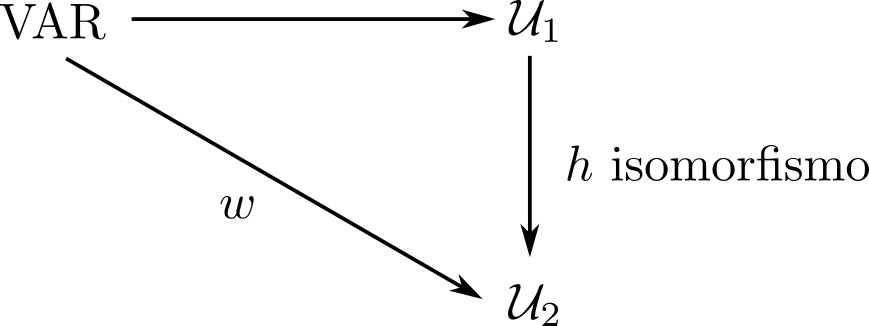
\includegraphics[width=0.58\textwidth]{corolario-aplicacion-iso-ida-1}
        \caption{Relación entre $\mathrm{VAR}$ y $\mathcal{U}_1$, 
        $\mathcal{U}_2$}
    \end{figure}
    ¿Cómo construimos una $v$ que satisfaga lo anterior? Aprovechando la
    biyectividad (en particular que es sobreyectiva):
    \begin{figure}[H]
        \centering
        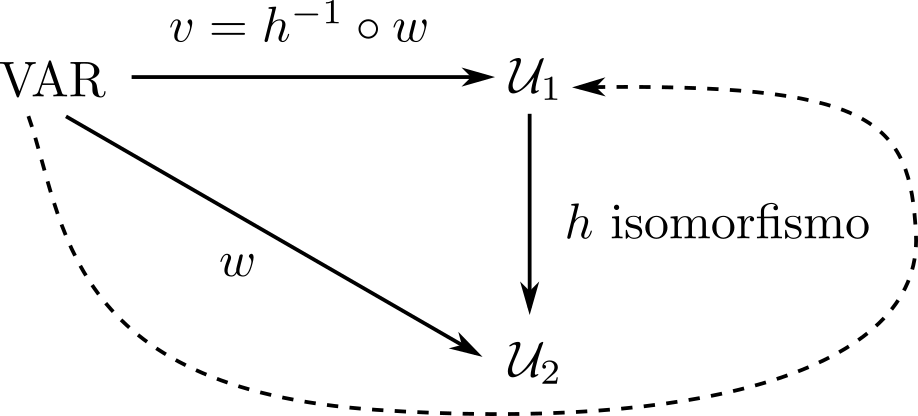
\includegraphics[width=0.58\textwidth]{corolario-aplicacion-iso-ida-2}
        \caption{Construcción de $v$.}
    \end{figure}
    Entonces $v$ es $v = h^{-1} \circ w$. Notemos que al aplicar $h$ 
    obtenemos $w$, que es precisamente lo que buscamos.

    Para la vuelta la idea es la misma: definimos $w = h \circ v$.
    \begin{figure}[H]
        \centering
        \includegraphics[width=0.58\textwidth]{%
            corolario-aplicacion-iso-vuelta}
        \caption{Construcción de $w$.}
    \end{figure}
    En ambos casos estamos usando el Teorema \ref{teo:equiv-isomorfs}:
    \begin{gather*}
        \mathcal{I}_1 \vDash \alpha[v] 
        \iff \mathcal{I}_2 \vDash \alpha [h \circ v] 
    \end{gather*}
\end{proof}

\subsubsection{Ejemplo}

$\mathcal{L}$ con $=$ y $f^2$. 
$\mathcal{I}_1 = (\mathbb{N}, +)$; $\mathcal{I}_2 = (\mathbb{N}, \, .)$

Probar que $\mathcal{I}_1 \not\approx \mathcal{I}_2$
\begin{gather*}
    \alpha = \exists \; x \quad \forall y \quad f^2 (x,y) = x
\end{gather*}

En $\mathcal{I}_1$:
\begin{align*}
    & \exists \; x \quad \forall y \quad x+y = x \\
    \iff & \exists \; x \quad \forall y \quad y = 0
\end{align*}

Falso. Basta tomar $y = 2$. $\implies V_{\mathcal{I}_1}(\alpha) = 0$

En $\mathcal{I}_2$:
\begin{align*}
    & \exists \; x \quad \forall y \quad x \, . \, y = x \\
    \iff & \exists \; x \quad \forall y \quad x(y-1) = 0
\end{align*}

Tomo $x = 0$ y es verdadero. $\implies V_{\mathcal{I}_2}(\alpha) = 1$

Luego
\begin{gather*}
    \underbrace{0 = V_{\mathcal{I}_1} (\alpha)}_{%
    \mathcal{I}_1 \text{ no es modelo de } \alpha}
    \neq 
    \underbrace{V_{\mathcal{I}_2} (\alpha) = 1}_{%
    \mathcal{I}_2 \text{ es modelo de } \alpha}
\end{gather*}

\begin{gather*}
    \therefore ~ \notamath{Por Corolario \ref{corol:no-equiv-isomorf} }
    \mathcal{I}_1 \not\approx \mathcal{I}_2
\end{gather*}

\medskip

\begin{corolario}{}{no-equiv-isomorf-2}
    Sea $\mathcal{L}$ de primer orden.

    Sea $\mathcal{I}$ interpretación de $\mathcal{L}$ 
    con universo $\mathcal{U}$.

    $F: \mathcal{U} \to \mathcal{U}$ isomorfismo.

    \medskip

    Entonces, si $a \in \mathcal{U}$ es distinguible $\implies F(a) = a$
\end{corolario}

¿Para qué nos sirve? Para probar que un elemento no es distinguible.

\begin{proof} \phantom{.}

    $a$ es distinguible 
    \nota{$a, b \in \mathcal{U}$}%
    $\implies$ $\exists \; \alpha(x) / 
    \underbrace{\overbrace{V_{\mathcal{I},v_{x=a}} (\alpha)= 1}^{%
    \circled{1}}}_{%
        \mathcal{I} \vDash \alpha [v_{x=a}]}$ y 
    $\overbrace{V_{\mathcal{I},v_{x=b}} (\alpha)= 0}^{\circled{2}}$ 
    si $b \neq a$.

    Aplicando el Teorema \ref{teo:equiv-isomorfs}:
    \begin{gather*}
        \mathcal{I} \vDash \alpha [F \circ v_{x=a}] \iff
        \notamath{$v$ ``manda'' $x$ a $a$, y
        al aplicarle $F$ lo ``manda'' a F(a)}
        \mathcal{I} \vDash \alpha [(F \circ v)_{x= F(a)}]
    \end{gather*}

    Esto nos está diciendo que $\alpha$ es verdadera en $\mathcal{I}$ cuando
    la valuación $(F \circ v)$ manda $x$ a $F(a)$.

    Además, por \circled{1} y \circled{2}, sabemos que la fórmula es verdadera
    en $y$ cuando $x = a$ y falsa cuando va a cualquier elemento distinto 
    de $a$.

    \begin{gather*}
        \therefore ~ F(a) = a
    \end{gather*}

\end{proof}

\subsubsection{Ejemplo}

Sea $\mathcal{L}$ con $=$ y $P^2$; $\mathcal{I} = (\mathcal{U}, \leq)$;
$\mathcal{U} = \{ a, b, c, d \}$.

\nota{$a \leq b$\\ $a \leq c$\\ $b \leq d$\\ $c \leq d$}%
\begin{figure}[H]
    \centering
    \includegraphics[width=0.40\textwidth]{%
    corolario-2-aplicacion-iso-ej-consigna}
    \caption{Relación de orden del universo.}
\end{figure}

Hallar los elementos distinguibles en $\mathcal{I}$.

\medskip

$a$ es distinguible porque
\begin{gather*}
    \alpha(x) = \forall y \quad P(x,y)\\
    V_{\mathcal{I}}(\alpha) = 1 \iff
    \forall y \quad x \leq y \implies \text{ en particular } x \leq a
    \implies x = a
\end{gather*}

Por otro lado $a \leq y ~ \forall y \implies V_{\mathcal{I}}(\alpha)=1$

Análogamente, $d$ es distinguible.
\begin{gather*}
    \beta(x) = \forall y \quad P(y,x)
\end{gather*}

\nota{$F$ es biyectiva.}%
Definimos $F: \mathcal{U} \to \mathcal{U} / F(a) = a; F(d) = d; F(b) = c
\text{ y }F(c) = b$.

Para ser un isomorfismo:
\begin{align*}
    x \leq y &\iff F(x) \leq F(y)\\
    a \leq b &\iff \underbrace{F(a)}_{a} \leq \underbrace{F(b)}_{c}\\
    a \leq a &\iff \underbrace{F(a)}_{a} \leq \underbrace{F(a)}_{a}\\
    a \leq d &\iff \underbrace{F(a)}_{a} \leq \underbrace{F(d)}_{d}\\
    \vdots
\end{align*}
En total son 9 renglones de desigualdades.

Una manera más corta es ayudándonos con los diagramas de Hasse.
\begin{figure}[H]
    \centering
    \includegraphics[width=0.45\textwidth]{%
    corolario-2-aplicacion-iso-ej-ans}
    \caption{Solución utilizando un diagrama de Hasse.}
\end{figure}

Como el diagrama es válido, se cumple $x \leq y \iff F(x) \leq F(y)$ y,
por lo tanto, $F$ es un isomorfismo.

En conclusión, como $F(b) \neq b$ $\implies b$ no es distinguible; y como
$F(c) \neq c$ $\implies c$ no es distinguible.


\bigskip
\textit{Noni:}
Notemos que con esto NO podemos probar que, como $F(a) = a$, entonces $a$ es
distinguible. El corolario es una implicación, no un sí y sólo sí.
Queda de tarea probar que la identidad siempre es un isomorfismo de $y$ en
$y$ con lo cual todos los elementos serían distinguibles, lo cual es falso
por lo que acabamos de demostrar.

Entonces para probar que los elementos son distinguibles, hay que encontrar
la fórmula que exprese el conjunto con dicho elemento. Para encontrar que
los elementos no son distinguibles, hay que encontrar un isomorfismo que
mueva dichos elementos.

\bigskip

\begin{corolario}{}{}
    Sea $\mathcal{L}$ un lenguaje de primer orden y sea $\mathcal{I}$ una
    interpretación de $\mathcal{L}$ con universo $\mathcal{U}$.

    Sea $F: \mathcal{U} \to \mathcal{U}$ un isomorfismo.

    \medskip

    Entonces
    \begin{gather*}
        \underbrace{F(A) \subseteq A}_{F(a) \, \in \, A ~ \forall a \in A}
        \quad \forall A \subseteq \mathcal{U}
    \end{gather*}
\end{corolario}

\begin{proof} \phantom{.}
    Tarea.

    Notemos que el corolario anterior es un caso particular de este.
\end{proof}

¿Para qué sirve? Para probar que un conjunto no es expresable.

\subsubsection{Ejemplo}

Sea $\mathcal{L}$ un lenguaje de 1\textsuperscript{er.} orden con $=$ y $f^2$.
Sea $\mathcal{I} = (\mathbb{Z}, +)$.

¿$A = \mathbb{N}$ es expresable?

\nota{Tarea: biyectiva}%
Defino $F: \mathbb{Z} \to \mathbb{Z} / F(x) = -x$
\begin{itemize}
    \item $F(x+y) = -(x+y) = -x + (-y) = F(x) + F(y)$
    \item $x = y \iff F(x) = F(y)$
\end{itemize}

Entonces $F$ es un isomorfismo.

Supongo $\mathbb{N}$ expresable $\implies F(\mathbb{N}) \subseteq \mathbb{N}$
pero $F(2) = -2 \notin \mathbb{N}$.
¡Absurdo!

\begin{center}
    $\therefore ~ A = \mathbb{N}$ no es expresable en $\mathcal{I}$.
\end{center}



\begin{corolario}{}{}
    Sea $\mathcal{L}$ un lenguaje de primer orden. 

    Sean $\mathcal{I}_1$ e $\mathcal{I}_2$ interpretaciones
     e $\mathcal{I}_1 \approx \mathcal{I}_2$.

    \medskip

    Si $a \in \mathcal{U}_1$ es distinguible en $\mathcal{I}_1$
    \begin{center}
        $\implies h(a) \in \mathcal{U}_2$ es distinguible en $\mathcal{I}_2$
    \end{center}
\end{corolario}

¿Para qué nos sirve? Para armar un isomorfismo.

\begin{proof} \phantom{.}

    Sabemos que: 
    \nota{Por el Teorema \ref{teo:equiv-isomorfs}}%
    $\mathcal{I}_1 \vDash \alpha[v] \overbrace{\iff}^{\star}
    \mathcal{I}_2 \vDash \alpha[h \circ v]$.

    Si $a \in \mathcal{U}_1$ es distinguible
    \begin{align*}
        &\implies \exists \; \alpha(x) \text{ que expresa } \{ a \} \\
        &\implies \mathcal{I}_1 \vDash \alpha(x)[v_{x=a}] \text{ y }
        \mathcal{I}_1 \not\vDash \alpha(x)[v_{x=b}] \text{ con } b \neq a\\
        &\implies \mathcal{I}_2 \vDash \alpha(x)[%
        \underbrace{h \circ v_{x=a}}_{{(h \circ v)}_{x = h(a)}}%
        ] \text{ y }
        \mathcal{I}_2 \not\vDash \alpha(x)[%
        \underbrace{h \circ v_{x=b}}_{{(h \circ v)}_{x = h(b)}}%
        ] 
        \text{ con } \underbrace{b \neq a}_{h(b) \neq h(a)} 
        \notamath{Por $\star$}
    \end{align*}

    \begin{center}
        $\therefore ~ \alpha(x)$ distingue $h(a)$ en $\mathcal{I}_2$.
    \end{center}
\end{proof}
